
\paragraph{Debuff} 
Spells specialized for crippling and weakening others. 


\subparagraph{Level 0} 
Common spells \\
\begin{tabular}{ m{3cm}m{14cm} } \hline
	\specialcell[p]{\textbf{Expelliarmus}         \\ 
\includegraphics[width=2.5cm]{../Pictures/Gameplay/Spells/Icon/Expelliarmus_spell_icon.png}}         & \begin{tabular}{p{14cm}} \textit{Forces whatever weapon an opponent is holding to fly out of their hand when attacking you.} \\ \hline Until the end of your next turn, you have resistance against bludgeoning, piercing, and slashing damage dealt by weapon attacks. \end{tabular} \\ \hline
\end{tabular}

\subparagraph{Level 1} 
Low level spells \\
\begin{tabular}{ p{3cm}p{14cm} } \hline
	\specialcell[p]{\textbf{Somnus}         \\ 
\includegraphics[width=2.5cm]{../Pictures/Gameplay/Spells/Icon/Somnus_spell_icon.jpg}}         & \begin{tabular}{p{14cm}} \textit{Produce a sweet sound that sends creatures into a magical slumber.} \\ \hline Roll 5d8; the total is how many hit points of creatures this spell can affect. Starting with the creature that has the lowest current hit points, each creature affected by this spell falls unconscious until the spell ends, the sleeper takes damage, or someone awakes the sleeper. Subtract each creature's hit points from the total before moving on to the creature with the next lowest hit points. A creature's hit points must be equal to or less than the remaining total for that creature to be affected. At Higher Levels: Roll an additional 2d8 for each slot level above 1st.\end{tabular} \\ \hline
	\specialcell[p]{\textbf{Petrificus}         \\ 
\includegraphics[width=2.5cm]{../Pictures/Gameplay/Spells/Icon/Petrificus_spell_icon.png}}         & \begin{tabular}{p{14cm}} \textit{Spell that temporarily paralyzes an humanoid opponent.} \\ \hline The target (humanoid) must succeed on a WIS saving throw or be paralyzed for the duration. At the end of each of its turns, the target can make another WIS saving throw. If successful, the spell ends on the target. At Higher Levels: You can target on additional humanoid for each slot level above 2nd. \end{tabular} \\ \hline
	\specialcell[p]{\textbf{Rictumsempra}         \\ 
\includegraphics[width=2.5cm]{../Pictures/Gameplay/Spells/Icon/Rictumsempra_spell_icon.jpg}}         & \begin{tabular}{p{14cm}} \textit{Tickles the target until they become weak with laughter.} \\ \hline The target must succeed on a WIS saving throw or fall prone, becoming incapacitated for the duration. A creature with an Intelligence score of 4 or less isn't affected. At the end of each of its turns, and each time it takes damage, the target can make another Wisdom saving throw. The target has advantage on the saving throw if it's triggered by damage. On a success, the spell ends. \end{tabular} \\ \hline
\end{tabular}                                                                                                                                 

\subparagraph{Level 3}                                                                                                                        
Medium spells \\                                                                                                                              
\begin{tabular}{ p{3cm}p{14cm} } \hline  
	\specialcell[p]{\textbf{Impedimenta} \\ 
\includegraphics[width=2.5cm]{../Pictures/Gameplay/Spells/Icon/Impedimenta_spell_icon.png}}         & \begin{tabular}{p{14cm}} \textit{Slows down or stops the target.} \\ \hline Change the time of up to 6 creatures on the field. Each target must succeed on a WIS saving throw or be have its speed is halved, a -2 penalty to AC and DEX saving throws, and it can't use reactions or multiattacks for the duration of the spell. 
	If the creature attempts to cast a spell with a casting time of 1 action, roll a d20. On an 11 or higher, the spell doesn't take effect until the creature's next turn, and the creature must use its action on that turn to complete the spell. If it can't, the spell is wasted. A creature affected by this spell makes another WIS saving throw at the end of each of its turns. On a successful save, the effect ends for it. \end{tabular} \\ \hline     
	\specialcell[p]{\textbf{Obscuro}                \\ 
\includegraphics[width=2.5cm]{../Pictures/Gameplay/Spells/Icon/Obscuro_spell_icon.png}}         & \begin{tabular}{p{14cm}} \textit{You can blind or deafen a foe.} \\ \hline Choose one creature to make a CON saving throw. If it fails, the target is either blinded or deafened  for the duration. At the end of each of its turns, the target can make a CON saving throw. On a success, the spell ends. At Higher Levels: You can target one additional creature for each slot level above 2nd. \end{tabular} \\ \hline     
	\specialcell[p]{\textbf{Weakening Hex}          \\ 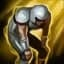
\includegraphics[width=2.5cm]{../Pictures/Gameplay/Spells/Icon/Weakening_spell_icon.jpg}}         & \begin{tabular}{p{14cm}} \textit{Cripple the spirits of the targets of this spell.} \\ \hline Up to six chosen creatures must make CHA saving throws. Whenever a target that fails this saving throw makes an attack roll or a saving throw before the spell ends, the target must roll a d4 and subtract the number rolled from the attack roll or saving throw. At Higher Levels: You can target one additional creature for each slot level above 1st. \end{tabular} \\ \hline                                                                                             
\end{tabular}                                                                                                                                 

\subparagraph{Level 5}                                                                                                                        
Greater spells \\                                                                                                                             
\begin{tabular}{ p{3cm}p{14cm} } \hline
	\specialcell[p]{\textbf{Confundo}           \\ 
\includegraphics[width=2.5cm]{../Pictures/Gameplay/Spells/Icon/Confundo_spell_icon.png}}         & \begin{tabular}{p{14cm}} \textit{Causes the victim to become confused and befuddled.} \\ \hline A target creature and its neighbours roll a d10: with a score of 1-6 the creatures take no action this turn, with a score of 7-8 the creatures make a melee attack against a random creature, with a score of 9-10 they can act normally. At the end of each of its turns, an affected target can make a Wisdom saving throw. If it succeeds, this effect ends for that target. \end{tabular} \\ \hline      
	\specialcell[p]{\textbf{Petrificus Totalus} \\ 
\includegraphics[width=2.5cm]{../Pictures/Gameplay/Spells/Icon/Petrificus_Totalus_spell_icon.png}}         & \begin{tabular}{p{14cm}} \textit{Spell that temporarily paralyzes any creature.} \\ \hline The target (creature) must succeed on a WIS saving throw or be paralyzed for the duration. At the end of each of its turns, the target can make another WIS saving throw. If successful, the spell ends on the target. At Higher Levels: You can target one additional creature for each slot level above 5th. \end{tabular} \\ \hline
\end{tabular}                                                                                                                                 

\subparagraph{Level 7}                                                                                                                        
Superior spells \\                                                                                                                            
\begin{tabular}{ p{3cm}p{14cm} } \hline
	\specialcell[p]{\textbf{Mantra}         \\ 
\includegraphics[width=2.5cm]{../Pictures/Gameplay/Spells/Icon/Mantra_spell_icon.png}}         & \begin{tabular}{p{14cm}} \textit{You repeat a mantra, imbued with malignant power.} \\ \hline Each chosen creature that can hear you must make a CHA saving throw. On a failed save, a creature suffers an effect based on its current hit points: 50hp (deafened for 1 turn), 40hp(deafened, blinded for 2 turns), 30hp (deafened, blinded, stunned for 3 turns), 20hp (killed). \end{tabular} \\ \hline                                                                                          
\end{tabular}

\subparagraph{Level 8} 
Supreme spells \\
\begin{tabular}{ p{3cm}p{14cm} } \hline
	\specialcell[p]{\textbf{Imperio}         \\ 
\includegraphics[width=2.5cm]{../Pictures/Gameplay/Spells/Icon/Imperio_spell_icon.png}}         & \begin{tabular}{p{14cm}} \textit{Places the victim completely under the caster's control.} \\ \hline You try to deceive a creature. He must succeed on a WIS saving throw or be charmed by you for the duration. If you or your partner are fighting him, he has the advantage on the saving throw. While charmed, the creature obeys the caster orders the best he can. Each time the target takes damage, it makes a new WIS saving throw against the spell. If the saving throw succeeds, the spell ends. \end{tabular} \\ \hline
\end{tabular}

\pagebreak
